\chapter{Design}

I udviklingsprocessen har der været fokus på at implementere hele features/user stories, og ikke enkelte lag af gangen. I en lagdelt arkitektur har det betydet at alle lag er blevet indraget i implementeringen af en given feature. I dette afsnit er det valgt at beskrive to features, for at eksemplificere selve designet af systemet. Disse er \textit{Oprette en bytteannonce} og \textit{Søg efter bytteannoncer}. For fuld beskrivelse af systemdesignet, se dokumentationen \footnote{Se bilag - Dokumentation, sektion 9}.

\section{Modeldesign}
I domæneanalysen blev der identificeret hvilke data, der er brug for at persistere. På figur \ref{fig:BarteradModel} A) kan Barterad-modellen\footnote{Barterad er en annonce på hjemmesiden}, som blev udarbejdet ud fra domæneanalysen, ses.

\begin{figure}[H]
	\centering
	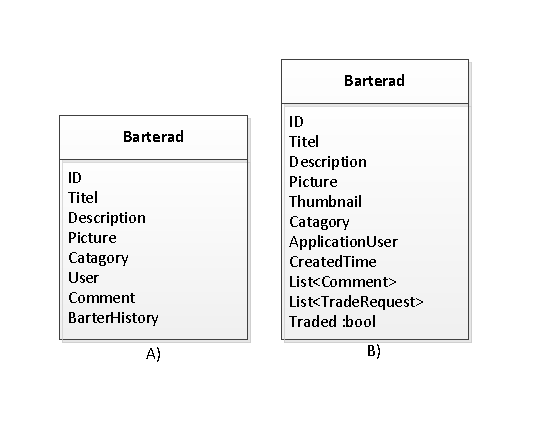
\includegraphics
	[width=140mm]{figures/BarterAdModels.pdf}
	\caption{A) BarterAd model fra domæneanalyse  B) Aktuel model}
	\label{fig:BarteradModel}
\end{figure} 

\noindent Der er blevet arbejdet agilt på projektet, og efter flere iterationer har designet ændret sig. På figur \ref{fig:BarteradModel} B ses det endelige modeldesign af BarterAds. \\ \\


\noindent Modellen oprettes igennem Entity Framework, og derefter tilgås dataene vha. et repository pattern. Dette pattern er anvendt fordi det standardiserer måden at tilgå data på, og det gør systemet mere testbart. Brugen af dette pattern uddybes i dokumentationen.\footnote{Se bilag - Dokumentation, sektion 9.8}


\section{Controllerdesign}  

I controllerne ligger selve funktionaliteten af BargainBarter systemet. Det er controllernes opgave at opdatere det view, som brugeren ser, samt styre kommunikationen mellem viewet og modellen. I dette afsnit forklares design og implementering af de controller actions der indgår i de valgte user stories.
 
\subsection{Oprette en bytteannonce}
Figur \ref{fig:SDOpretBarterAd} viser et scenarie, hvor brugeren opretter en ny annonce. Brugeren trykker på knappen \textit{Ny annonce}, hvilket systemet registrerer, og kalder den tilhørende action. Igennem denne action returneres \textit{Create BarterAd} viewet. I dette view kan der indtastes data til Barterads. Brugeren indtaster data og trykker \textit{Opret}, hvorved controlleren opretter og persisterer Barterad'en udfra de indtastede data.  \\


\begin{figure}[H]
	\centering
	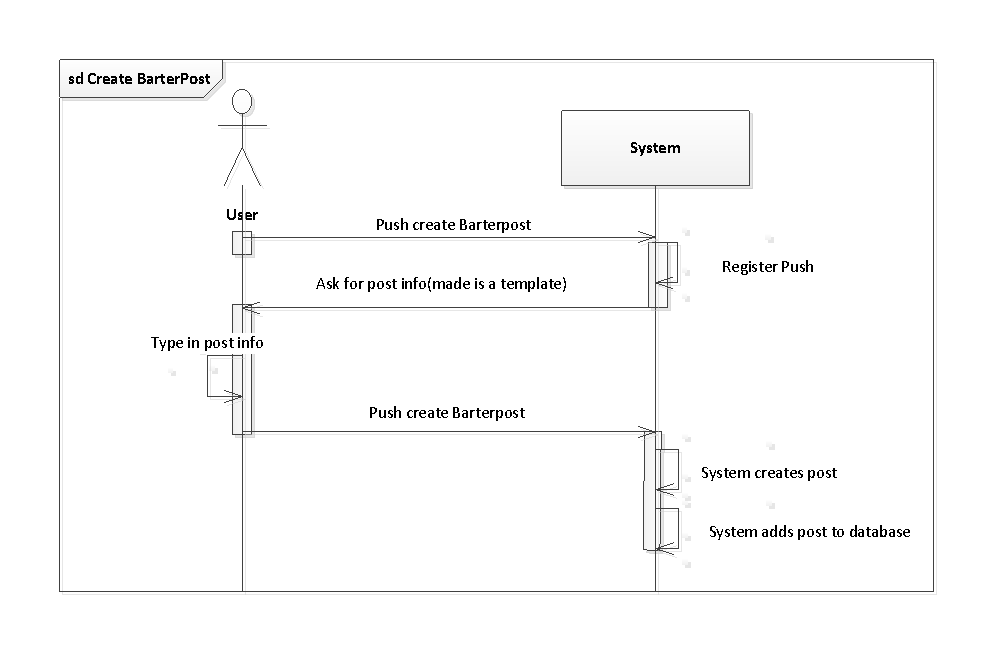
\includegraphics
	[width=140mm]{../Dokumentation/figures/SDOpretBytteAnnonce.PDF}
	\caption{Sekvensdiagram for oprettelse af barterads}
	\label{fig:SDOpretBarterAd}
\end{figure}

\noindent Beskrivelse af annonceoprettelse er en ''happy path'' beskrivelse, som ikke tager højde for fejl. I design og implementering af alle controllers bliver der håndteret mulige fejl. For eksempel kan man ikke oprette en annonce uden at være logget ind. Dette holder controlleren styr på. 

\subsection{Søg efter bytteannoncer}     
På hjemmesiden kan der søges efter annoncer på flere måder. Det kan være på kategori, titel og på afstand. I dette eksempel uddybes søgning efter annoncer filtreret efter afstand. Desuden eksemplificerer implementeringen af denne feature den generelle virkemåde af samspillet mellem lagene i systemet. 

\subsubsection{Valg af løsning}
Der blev i forundersøgelsen til denne feature overvejet flere løsningsmuligheder. Der var mulighed for at få eksempelvis Google Maps API\cite{googleapi} til at lave en ruteplan, og ud fra den bestemme afstanden til andre brugere. Denne løsning var ikke optimal af flere årsager. For det første kunne det blive meget performance-tungt at lave alle de forespørgsler til Google Maps API. For det andet kunne der let opstå begrænsninger ift. de maksimale antal forespørgsler som Google Maps API tillader. For det tredje blev det vurderet, at det ikke var nødvendigt med meget høj præcision på afstanden til en annonces ejer.  \\

\noindent En anden løsning der var på tale, var blot at sortere efter postnumre. Dette blev dog vurderet til at være for upræcist, da arealet af et postnummer kan være meget stort. 
\\

\noindent Løsningen som blev udtænkt baserer sig på beregning af afstand i fugleflugt mellem koordinater. Ved oprettelse af en brugerprofil indtaster brugeren en adresse. Vha. Google Maps API udtrækkes koordinater baseret på adressen, og disse koordinater gemmes som attributter på modellen for en bruger. Selve beregningen af afstand fungerer som en trigonometrisk udregning. Det blev valgt at anvende Google Maps API fremfor andre API'er, fordi gruppen synes det kunne være spændende at anvende et af Googles mange API'er, og det ville være relevant at få erfaring med ét af disse. Denne løsning er et godt kompromis mellem høj præcision, performance og overskuelig implementering.

\subsubsection{Implementering}
\noindent Selve søgefunktionen kaldes fra et UI\footnote{User Interface} element i form af en slider. Denne kan ses på figur \ref{fig:slider}. 

\begin{figure}[H]
	\centering
	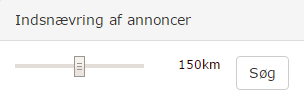
\includegraphics
	[width=90mm]{figures/slider.png}
	\caption{Slider til søgning filtreret efter afstand}
	\label{fig:slider}
\end{figure}

\noindent Actionen eager loader\footnote{Ved eager loading forstås der at når man laver forespørgsel på en entitet, så loades der relateret entiter i samme forespørgsel} alle Barterads, og adresser på brugerne. Desuden loades brugerens egne koordinater. Derefter udregnes afstanden mellem brugeren selv og de resterende brugere. Alle der er inden for den valgte afstand på slideren bliver gemt i en liste. Derefter findes alle de gemte brugeres Barterads, der ikke allerede er byttet. Disse bliver returneret sammen med frontpage viewet, så resultatet af søgningen kan præsenteres. Denne funktionalitet giver mulighed for, at man kan finde de Barterads der ligger tæt på brugeren. Scenariet her er ligeledes beskrevet som "happy path", hvor situationer som fx. at brugeren ikke er logget ind ikke benævnes.

\section{Viewdesign}

Viewet sørger for selve det visuelle udtryk af hjemmesiden, og er præsentationslogikken i systemet. Det bestræbes at undgå at lægge businesslogik i viewet, således at præsentationslaget i højst mulig grad er afkoblet fra resten af systemet. I dette afsnit beskrives design og implementering af views for de valgte user stories.

\subsection{Oprette en bytteannonce}
Viewet for oprettelsen af en bytteannonce er et meget typisk eksempel på opbygningen af et view. Viewet består af en form, der mapper nogle data til en bestemt post action i controlleren, ved tryk på en submit-knap. Denne post action behandler så disse data. Desuden validerer viewet at alle datafelter er udfyldte, og fortæller brugeren hvad han/hun mangler at udfylde. Figur \ref{fig:postview} illustrerer et eksempel på hvordan en form mapper til en bestemt action i en controller.

\begin{figure}[H]
	\centering
	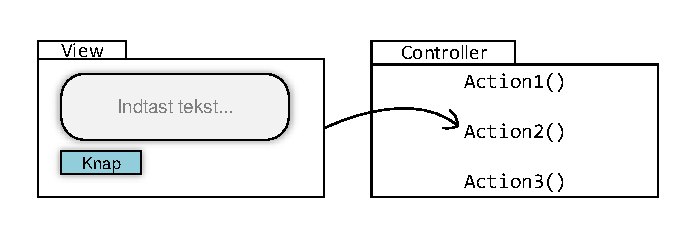
\includegraphics
	[width=140mm]{figures/viewtocontroller.pdf}
	\caption{Eksempel på form}
	\label{fig:postview}
\end{figure}

\subsection{Søg efter bytteannoncer}
Søgning efter bytteannonce har ikke et separat view, men er et delelement af viewet for forsiden. I forbindelse med implementering af søgning, krævede det en tilføjelse af slideren som ses i figur \ref{fig:slider}. Denne slider fungerer således som en form på samme måde som i det view, hvor der kan der kan oprettes bytteannoncer. Dette betyder at der skal vælges en bestemt værdi ved brug af slideren, og dernæst trykkes søg. Målet var at implementere denne feature med en postback-metode, som ville gøre, at resultatet blev vist dynamisk. Denne løsning var der dog ikke tid til at implementere.
